\chapter{Movimentação}
\section*{Introdução}
    \paragraph{}
    Será neste capítulo que iremos aprender a movimentar o \textsl{Sparki}, os comandos para ele ir para frente, rotacionar e realizar todos os percursos que a nossa imaginação puder criar. Para isso, será necessário utilizar as funções a seguir.
    
\section{Funções}
    \paragraph{}
    Todas as funções desse capítulo começam com \lstinline[columns=fixed]{sparki.move}, você consegue pensar em um motivo para a palavra ``move'' estar em destaque?\\
    
    \textit{Move... Mover... Movimentar...} \par
    Exatamente! Movimentação é a resposta, pois ``move'' significa ``se movimentar'' em inglês.

\subsection{sparki.moveForward(int distancia);}
    \paragraph{}
    Essa é a principal função de movimentação, pois é um comando para o robô ``andar'' para frente. Sendo ``distancia'' uma variável que representa quantos centímetros o \textsl{Sparki} deverá se movimentar para frente. Após ter percorrido essa distância, ele passará a executar a próxima linha de comando, ou seja, a próxima ação.\\
    
    \textit{Variável? Mas o que é essa tal de variável?} \par
    Não se preocupe! Teremos um capítulo inteiro apenas para entendê-la, mas, por enquanto, iremos utilizá-la para informar ao \textsl{Sparki} qual a distância em centímetros que queremos que ele percorra, ou os ângulos em graus que queremos que ele rotacione. Simples assim!\\
    
    \textit{E o que significa esse `int' dentro dos parênteses?} \par
    Ele indica que o número que colocaremos dentro dos parênteses tem que ser um número inteiro.
    
    \begin{center}
    \textcolor{mydarkblue!80!black}{\textbf{Lembrando:}} Números inteiros são aqueles que não têm a parte decimal, ou seja, não possuem vírgula. $\mathbb{Z}=\{..., -3, -2, -1, 0, 1, 2, 3, ...\}$.
    \end{center}
    
    \paragraph{}
    Como queremos que o \textsl{Sparki} vá para frente, além de ser um número inteiro, tem que ser positivo também! Ah! Se não tiver escrito nada no espaço entre os parênteses, o \textsl{Sparki} irá para frente indefinidamente, ou seja, até que seja lida a função \lstinline[columns=fixed]{sparki.moveStop()}, ou até que a bateria dele acabe...
    \paragraph{}
    Parece complicado, mas vou dar um exemplo passo a passo para você ver que não é.
    \\~\\
    \textsc{Exemplo 1)} Vamos supor que o seu objetivo é fazer o \textsl{Sparki} andar para frente.
    
    \begin{itemize}
        \item O primeiro passo é identificar a função a ser utilizada para o \textsl{Sparki} andar para frente, neste caso, \lstinline[columns=fixed]{sparki.moveForward(int distancia)};
        \item O segundo passo é decidir o qual vai ser o valor a ser escrito entre os parênteses, ou seja, o parâmetro dessa função. Como não determinamos uma distância, pois queremos que ele ande para frente e não pare, não é necessário escrever um número, basta deixar em branco. O valor default é 1, logo, escrever \lstinline[columns=fixed]{sparki.moveForward()} é o mesmo que escrever \lstinline[columns=fixed]{sparki.moveForward(1)};
        \item Agora que sabemos a função e o seu parâmetro, podemos aplicar no código. Ficaria assim:
    \end{itemize}
    
    \begin{lstlisting}[language=C]
#include <Sparki.h>;

void setup()
{
}

void loop()
{
    sparki.moveForward();
}
\end{lstlisting}
    
    \paragraph{}
    Quando queremos passar uma informação para outra pessoa, podemos falar de diversas formas, seja de um jeito mais devagar ou até muito rápido, bem formal ou com várias gírias. Então, pode-se dizer que, independente do modo com que falamos, a pessoa irá entender a informação, mas, dependendo da pessoa com quem falamos, devemos escolher o modo mais conveniente. Por exemplo, não podemos falar da mesma forma com os nossos amigos e com o/a diretor/a do colégio, para este último devemos tentar utilizar uma linguagem mais formal. Na programação isso também acontece, existem vários códigos diferentes que fazem basicamente a mesma coisa, mas sempre devemos escolher o mais eficiente ou conveniente para cada caso.
    \\~\\
    \textsc{Exemplo 2)} Vamos aproveitar para ver um código que faz o mesmo que o do \textsc{Exemplo 1}. Outra forma de fazer o robô andar para frente sem parar seria escrevendo um número qualquer como parâmetro \lstinline[columns=fixed]{sparki.moveForward(int distancia)}.
    
    \begin{lstlisting}[language=C]
#include <Sparki.h>;

void setup()
{
}

void loop()
{
    sparki.moveForward(100);
}
\end{lstlisting}
    
    \textit{Como assim?? Você disse que o número que vinha dentro dos parênteses determinava a distância. Então, se eu colocar um número qualquer, o \textsl{Sparki} vai parar depois de andar a distância escrita, não?} \\
    Sim, o número dentro dos parênteses indica sim a distância a ser percorrida, mas há algo que você pode estar se esquecendo. Tente se lembrar da definição de \lstinline[columns=fixed]{void loop()}. Ela falava que tudo o que estiver escrito dentro das chaves do \lstinline[columns=fixed]{void loop()} seria repetido várias e várias vezes, até que a bateria do robô acabe. Como só existe uma função dentro do loop, essa vai se repetir para sempre, é como se o \textsl{Sparki} estivesse andando 100 centímetros para frente e, depois que terminasse, mais 100 centímetros para frente e depois mais 100 centímetros para frente... Essa sequência ficaria se repetindo, sem parar.
    
    \paragraph{}
    Bom, chegamos a conclusão de que o \textsc{Exemplo 1} e o \textsc{Exemplo 2} são códigos que geram a mesma ação, agora devemos pensar em qual seria mais eficiente ou conveniente na hora de escrever. Geralmente, optamos pelo código mais simples, sem elementos desnecessários, para que quem estiver lendo possa compreender melhor o nosso código. Logo, o \textsc{Exemplo 1} seria a melhor escolha.
    
    \begin{center}
    \textcolor{mydarkblue}{\textbf{Para não esquecer!}} \\``Forward'' traduzido para o português significa ``para frente''. 
    \end{center}

\subsection{sparki.moveBackward(int distancia);}
    \paragraph{}
    Parecida com a anterior, essa função é utilizada para que o \textsl{Sparki} ``ande'' para trás, sem fazer giros. Sendo ``distancia'' uma variável que representa quantos centímetros ele deverá se movimentar para trás. Da mesma forma que o \lstinline[columns=fixed]{sparki.moveForward()}, se não for escrito nada no espaço entre os parênteses, o \textsl{Sparki} irá para trás indefinidamente, ou seja, até que seja lida a função \lstinline[columns=fixed]{sparki.moveStop()}.
    \\~\\
    
    \textsc{Exemplo 1)} Nesse exemplo, veremos um código que faz o \textsl{Sparki} andar 1 metro para frente e 1 metro para trás.
    
    \begin{itemize}
        \item As funções necessárias são: \lstinline[columns=fixed]{sparki.moveForward(int distancia)}, para andar para frente, e \lstinline[columns=fixed]{sparki.moveBackward(int distancia)}, para andar para trás;
        \item A distância é de 1 metro, mas como o valor tem que ser em centímetro, devemos transformar de metro para centímetros. Substituindo os parâmetros, as funções ficariam assim: \lstinline[columns=fixed]{sparki.moveForward(100)}, \lstinline[columns=fixed]{sparki.moveBackward(100)}.
        \item Agora é só escrever em forma de código!
    \end{itemize}
    
    \begin{lstlisting}[language=C]
#include <Sparki.h>;

void setup()
{
}

void loop()
{
    sparki.moveForward(100);
    sparki.moveBackward(100);
}
\end{lstlisting}
    
    \paragraph{}
    Também poderíamos inserir a função \lstinline[columns=fixed]{delay(int tempo)} entre as funções de movimentação para que o \textsl{Sparki} realize melhor esses movimentos.\\
    
    \textit{O que essa função \lstinline[columns=fixed]{delay(int tempo)} faz mesmo?} \par
    Ela estabelece um tempo de intervalo entre as ações, simplificando, o \textsl{Sparki} espera um tempo determinado pela variável ``tempo'' antes de executar a próxima ação, com isso, podemos acompanhar melhor a execução dos movimentos que escrevemos no nosso código.\\
    
    \textsc{Exemplo 2)} Agora, iremos reescrever o código anterior utilizando a função \lstinline[columns=fixed]{delay(int tempo)} para que, antes do \textsl{Sparki} mudar o sentido do seu movimento, ele dê uma pausa de 3 segundos.
    
    \begin{lstlisting}[language=C]
#include <Sparki.h>;

void setup()
{
}

void loop()
{
    sparki.moveForward(100);
    delay(3000);
    sparki.moveBackward(100);
    delay(3000);
}
\end{lstlisting}
    
    \textit{Por que existem dois \lstinline[columns=fixed]{delay(3000)} no código?}
    
    O primeiro é necessário para estabelecer um intervalo entre andar para frente e andar para trás. O segundo serve para estabelecer um intervalo entre andar para trás e andar para frente, porque, como as funções estão dentro do \lstinline[columns=fixed]{void loop}, depois de \lstinline[columns=fixed]{sparki.moveBackward(100)} o próximo movimento seria \lstinline[columns=fixed]{sparki.moveForward(100)}, então, devemos colocar uma pausa ali também.  
    
    \begin{center}
        \textcolor{mydarkblue!80!black}{\textbf{Lembrando:}} No exemplo anterior nós utilizamos a palavra ``sentido'' no enunciado. Mas você se lembra o que realmente significa esse conceito? E qual a diferença entre ``sentido'' e ``direção''? Vou dar um exemplo para você não errar mais na hora de diferenciar os dois.
    \end{center}
    
    \paragraph{}
    Vamos supor que você saiu de casa e ficou perdido no meio da cidade apenas com a sua pulseira da sorte e uma bússola para te auxiliar a voltar para casa. Essa bússola vai indicar a direção sul, norte, leste, oeste e as várias direções de acordo com os 360 graus dela. Você tem o conhecimento de que a sua casa fica para o sul, por isso, começa a andar nessa direção, saindo da cidade e indo para sua casa. Alguns minutos depois você chega ao seu destino, mas percebe que a sua pulseira caiu no meio do caminho. Então você decide ir de novo para a cidade, pela mesma direção que você veio na volta, mas no sentido contrário ao que você utilizou para voltar para casa, ou seja, saindo da sua casa e indo para a cidade. 
    \paragraph{}
    Contada a história, vamos refletir. A direção pode ser simplificada como uma reta que liga a cidade à sua casa e esta reta possui dois sentidos, o de ida e o de volta. Então, quando estamos falando de uma direção, para facilitar, imagine uma linha tracejada entre o local inicial e o seu ponto de destino. Quando estamos falando de sentidos, pense nessa linha como uma seta (casa -> cidade) para a ida e (cidade -> casa) para a volta.

    \begin{center}
    \textcolor{mydarkblue}{\textbf{Para não esquecer!}} \\ ``Backward'' traduzido para o português significa "para trás".
    \end{center}
    
    \begin{figure}[h]
    \caption{Movimentação Básica}
     
    \centering 
    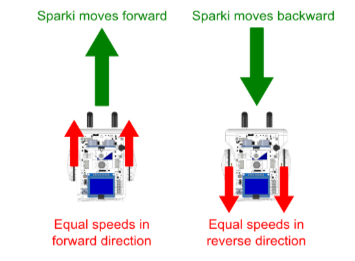
\includegraphics[width=9cm]{Figuras/movimentation_for_back.png}
    \label{figura:movimentation_for_back.png}
    \end{figure}
    
\subsection{sparki.moveStop();}
    \paragraph{}
    Esse é um comando para o \textsl{Sparki} parar de se movimentar, independente do que ele estiver fazendo. Observe que não é necessário escrever nada dentro dos parênteses, o robô irá parar de realizar a ação que ele estiver fazendo no momento em que esse comando for lido.
    
    \begin{center}
        \textcolor{mydarkblue!80!black}{\textbf{Lembrando:}} O tempo a ser escrito como parâmetro, dentro dos parênteses, deve estar em milissegundos.
    \end{center}
    
    \textsc{Exemplo 1)} Neste próximo exemplo, faremos o \textsl{Sparki} andar para frente por 2 segundos e parar, repetidamente.
    
    \begin{itemize}
        \item Primeiro vamos identificar as funções a serem utilizadas para o \textsl{Sparki} andar para frente, esperar 2 segundos e parar. Como vimos no exemplo anterior, a função \\ \lstinline[columns=fixed]{sparki.moveForward(int distancia)} será responsável por andar para frente. Para esperar 2 segundos, devemos utilizar a função \lstinline[columns=fixed]{delay(int tempo)}. Por último, utilizaremos a função \lstinline[columns=fixed]{sparki.moveStop()}, com o objetivo de fazer o \textsl{Sparki} parar.
        \item Agora, vamos decidir os parâmetros dessas 3 funções. Como queremos que o robô ande durante 2 segundos, a função \lstinline[columns=fixed]{sparki.moveForward(int distancia)} será escrita antes da \lstinline[columns=fixed]{sparki.moveStop()}. O \textsl{Sparki} deverá andar por 2 segundos, logo, essa função deverá ser escrita entre as duas anteriores.
        \item Aplicando em código temos:
    \end{itemize}
    
    \begin{lstlisting}[language=C]
#include <Sparki.h>;

void setup()
{
}

void loop()
{
    sparki.moveForward();
    delay(2000);
    sparki.moveStop();
}
\end{lstlisting}
    
    O uso da função \lstinline[columns=fixed]{delay(int tempo)} é de suma importância para o movimento funcionar, sem ela, as funções de andar para frente e parar entrarão em conflito.
    
    \begin{center}
    \textcolor{mydarkblue}{\textbf{Para não esquecer!}}
    \\``Stop'' traduzido para o português significa ``Parar''.
    \end{center}
    
\subsection{sparki.moveRight(int graus);}

    \paragraph{}
    Um pouco diferente dos anteriores, esse é um comando de girar para a direita. Sendo ``graus'' uma variável que representa a variação em graus do giro. Se este campo ficar em branco, o \textsl{Sparki} executará um giro de 90° para a direita.
    \\~\\
    
    \begin{figure}[h]
    \caption{Rotação do Sparki}
     
    \centering 
    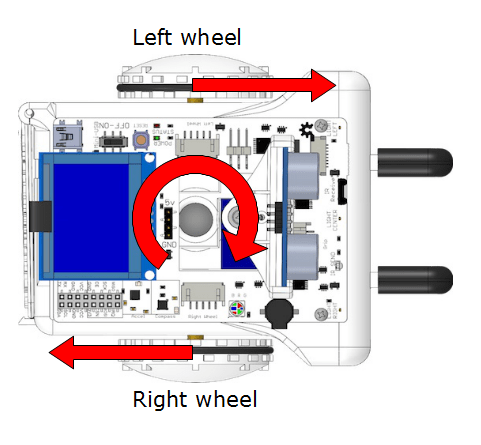
\includegraphics[width=7cm]{Figuras/rotation.png}
    \label{figura:rotation.png}
    \end{figure}
    
    \textsc{Exemplo 1)} Neste código, o \textsl{Sparki} executará um giro à direita de 90° e ficará parado por 1 segundo antes de executar novamente o giro.
    
    \begin{itemize}
        \item As funções necessárias são: \lstinline[columns=fixed]{sparki.moveRight(int graus)} para girar para a direita e \lstinline[columns=fixed]{delay(int tempo)} para gerar uma pausa;
        \item Substituindo os parâmetros, as funções ficariam assim: \lstinline[columns=fixed]{sparki.moveRight()}, pois 90° é o mesmo que deixar em branco, e \lstinline[columns=fixed]{delay(1000)}.
        \item Escrevendo em forma de código:
    \end{itemize}
    
    \begin{lstlisting}[language=C]
#include <Sparki.h>;

void setup()
{
}

void loop()
{
    sparki.moveRight();
    delay(1000);
}
\end{lstlisting}
    
    \begin{center}
    \textcolor{mydarkblue}{\textbf{Para não esquecer!}}
    \\``Right'' traduzido para o português significa ``Direita'', mas lembre-se que não é um deslocamento para direita, e sim um giro.
    \end{center}
    
\subsection{sparki.moveLeft(int graus);}
    \paragraph{}
    Esta função é responsável pelo giro para a esquerda do \textsl{Sparki}. Sendo ``graus'' uma variável que representa a variação em graus do giro. Se este campo ficar em branco, o \textsl{Sparki} executará um giro de 90° para a esquerda.
    \\~\\
    \textsc{Exemplo 1)} Neste exemplo, nós criaremos um código que fará o \textsl{Sparki} realizar um giro completo para a direita, esperar 1 segundo, realizar um giro completo para a esquerda e esperar mais 1 segundo antes que ele repita a sequência.
    
    \begin{itemize}
        \item As funções necessárias são: \lstinline[columns=fixed]{sparki.moveRight(int graus)} para girar para a direita, \lstinline[columns=fixed]{sparki.moveLeft(int tempo)} para girar para a esquerda, além da \lstinline[columns=fixed]{delay(int tempo)} para o intervalo;
        \item Para completar um giro, é necessário realizar os 360 graus, por isso, esse número deve ser escrito dentro dos parênteses das funções de girar. Com o objetivo de fazer uma pausa de 1 segundo, devemos escrever 1000 dentro dos parênteses da função de pausa. Substituindo os parâmetros, as funções ficariam assim: \lstinline[columns=fixed]{sparki.moveRight(360)}, \lstinline[columns=fixed]{sparki.moveLeft(360)}, \lstinline[columns=fixed]{delay(1000)}.
        \item Escrevendo em forma de código:
    \end{itemize}
    
    \begin{lstlisting}[language=C]
#include <Sparki.h>;

void setup()
{
}

void loop()
{
    sparki.moveRight(360);
    delay(1000);
    sparki.moveLeft(360);
    delay(1000)
}
\end{lstlisting}

    \textsc{Exemplo 2)} Que tal juntarmos a função de andar para frente e girar para a esquerda? O código a seguir faz \textsl{Sparki} ir e voltar em uma linha reta. Os movimentos passo a passo são os seguintes: ir para frente por 0,1 metro, esperar 1 segundo parado, girar para a esquerda 180 graus e esperar 1 segundo parado antes de repetir.

\begin{lstlisting}[language=C]
#include <Sparki.h>;

void setup()
{
}

void loop()
{
    sparki.moveForward(10);
    delay(1000);
    sparki.moveLeft(180);
    delay(1000)
}
\end{lstlisting}
    
    \begin{center}
   \textcolor{mydarkblue}{\textbf{Para não esquecer!}}
   \\``Left'' traduzido para o português significa ``Esquerda'', mas lembre-se que não é um deslocamento para esquerda e sim um giro.
    \end{center}
    
    \begin{figure}[h]
    \caption{Sparki fazendo uma curva}
     
    \centering 
    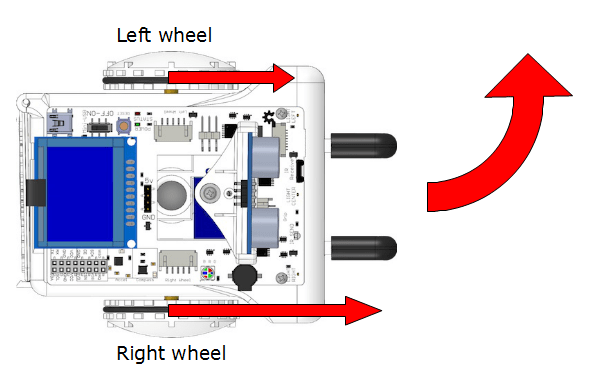
\includegraphics[width=7cm]{Figuras/movingTheRobotmoveLeft.png}
    \label{figura:movingTheRobotmoveLeft.png}
    \end{figure}
    
\subsection{sparki.motorRotate(int motor, int direcao,  int velocidade);}

Quer aprofundar um pouco mais o seu conhecimento sobre movimentação? Então vamos nessa!
\paragraph{}
Sabemos que o \textsl{Sparki} possui duas rodas, mas, para que elas possam rotacionar e fazer o robô se movimentar, tem que existir algo gerando um movimento de rotação. E quem se ocupa dessa tarefa é o motor. Como são duas rodas, existem dois motores, um do lado de cada roda. Para padronizar, iremos chamar o motor do lado direito de ``MOTOR\_RIGHT'' e o motor do lado esquerdo de ``MOTOR\_LEFT''. Agora já sabemos que tem um motor para gerar o movimento, mas, além disso, é necessário decidimos mais duas coisas: qual será a direção para onde ele irá girar e qual será a velocidade dessa rotação. Exitem duas direções de rotação, uma seria o sentido horário e outra o sentido anti-horário, elas serão chamadas respectivamente de: ``DIR\_CW'' e ``DIR\_CCW''.
\paragraph{}
Pronto! Acabamos de aprender os três parâmetros necessários para utilizar a função \lstinline[columns=fixed]{sparki.motorRotate(int motor, int direção, int velocidade)}. No lugar da variável ``motor'' utilizaremos ``MOTOR\_RIGH' se quisermos movimentar o motor e, consequentemente, a roda direita ou ``MOTOR\_LEFT'' se quisermos movimentar a roda esquerda. E no lugar variável ``direcao'' devemos escrever ``DIR\_CW'', sentido do relógio, ou ``DIR\_CCW'', sentido contrário ao do relógio, mas temos que escolher esses dois com cuidado, pois os motores estão virados para fora. Por exemplo, para o motor direito andar para frente, ele utiliza o sentido do relógio, já para o esquerdo, deve-se utilizar o sentido contrário ao do relógio.\\

\textit{Não entendi nada... Se as duas rodas devem andar para frente, por quê um motor utiliza o sentido do relógio e o outro o contrário dele?}\par
Porque o parâmetro ``direcao'' não se refere à direção para onde as rodas estão indo, e sim para que sentido elas estão girando. Tente imaginar o \textsl{Sparki} desmontado, o motor da esquerda estará apontando para a esquerda e o motor da direita estará pontando para a direita, por esse motivo, as direções de rotações serão invertidas. 
\paragraph{}
Faça o teste: vamos supor que os seus dedos são as rodas e as suas mãos os motores. Cruze as mãos e aponte o dedo da mão direita para a direita e o dedo da mão esquerda para a esquerda, olhe no sentido de fora para dentro (ponta da unha -> mão) de cada dedo e gire os dedos no sentido do relógio. Ao fazer o movimento, você perceberá que se o seu dedo que aponta para a direita fosse uma roda, ela estaria andando para frente, mas, se o seu dedo que aponta para a esquerda fosse uma roda, esta estaria andando para trás.
\paragraph{}
Já a terceira variável, ``velocidade'', deve ser substituída por um número entre 0 e 100, sendo 0 a velocidade mínima e 100 a velocidade máxima.
\\~\\
\textsc{Exemplo 1)} Agora um exemplo bem simples para você entender. Utilizaremos a função de rotação do motor para realizar uma ação semelhante à que fizemos no início do capítulo: fazer o \textsl{Sparki} andar para frente por um tempo indeterminado.
        
\begin{itemize}
    \item A função a ser utilizada é \lstinline[columns=fixed]{sparki.motorRotate(int motor, int direcao, int } \\ \lstinline[columns=fixed]{velocidade)}.
    \item Devemos prestar bastante atenção neste momento. Nosso objetivo é fazer o \textsl{Sparki} andar para frente, logo, o motor da direita, ``MOTOR\_RIGHT'', deverá rotacionar no sentido do relógio, ``DIR\_CW'', enquanto o motor da esquerda, ``MOTOR\_LEFT'', deverá rotacionar no sentido contrário ao do relógio, ``DIR\_CCW''. E o parâmetro \lstinline[columns=fixed]{int velocidade} pode ser 75.
    \item Ficará assim:
\end{itemize}
    
    \begin{lstlisting}[language=C]
#include <Sparki.h>;

void setup()
{
}

void loop()
{
    sparki.motorRotate(MOTOR_LEFT, DIR_CCW, 75);
    sparki.motorRotate(MOTOR_RIGHT, DIR_CW, 75);
}
\end{lstlisting}

\begin{center}
    \textcolor{mydarkblue!80!black}{\textbf{Lembrando:}} Em Física, sempre devemos falar de velocidade especificando a unidade de medida, com base no Sistema Internacional de unidades (SI). No caso da velocidade do \textsl{Sparki}, estamos nos referindo a uma porcentagem da velocidade máxima que pode ser atingida por ele. Por exemplo, se a velocidade for 50, na realidade, estaríamos nos referindo à 50\% da velocidade máxima, por isso, não há necessidade de colocarmos a unidade de medida.
\end{center}

\textsc{Exemplo 2)} Vamos complicar um pouquinho mais, que tal? Dessa vez, o \textsl{Sparki} irá executar um movimento de ondulação (de cobrinha) e, para isso, vamos colocar os dois motores andando para frente, o da direita com uma velocidade maior que o da esquerda e depois de 5 segundos, o da esquerda com uma velocidade maior que o da direita. Assim, ele estará rotacionando levemente para a esquerda ao mesmo tempo que continua andando e, após o tempo que determinamos, ele estará rotacionando levemente para a direita e andando. Como essas ações estão no \lstinline[columns=fixed]{void loop()}, elas se repetirão várias e várias vezes, formando um movimento de ondulação.

    \begin{lstlisting}[language=C]
#include <Sparki.h>;

void setup()
{
}

void loop()
{
    sparki.motorRotate(MOTOR_LEFT, DIR_CCW, 50);
    sparki.motorRotate(MOTOR_RIGHT, DIR_CW, 100);
    
    delay(5000);
    
    sparki.motorRotate(MOTOR_LEFT, DIR_CCW, 100);
    sparki.motorRotate(MOTOR_RIGHT, DIR_CW, 50);
    
    delay(5000);
}
\end{lstlisting}

\begin{center}
    \textcolor{mydarkblue}{\textbf{Para não esquecer!}}
    \\``CW'' de ``DIR\_CW'' é uma abreviação para ``clockwise'', que se refere ao sentido do relógio. ``CCW'' de ``DIR\_CCW'' é uma abreviação para ``counterclockwise'', que se refere ao sentido contrário ao do relógio.
\end{center}

\subsection{sparki.motorStop(int motor);}
\paragraph{}
Esta função é semelhante à \lstinline[columns=fixed]{sparki.moveStop()} apresentada no início do capítulo, mas, ao invés de \lstinline[columns=fixed]{move}, está escrito \lstinline[columns=fixed]{motor} pois estamos nos referindo ao motor do \textsl{Sparki}. Ela deve ser utilizada em conjunto com a função \lstinline[columns=fixed]{sparki.motorRotate(int motor, int direcao, int velocidade)} para informar ao motor a ordem de parada. O parâmetro \lstinline[columns=fixed]{int motor} serve para informar qual motor que você deseja parar ( ``MOTOR\_RIGH'' ou ``MOTOR\_LEFT'').
\\~\\
\textsc{Exemplo 1)} Dessa vez, iremos utilizar a função de rotação e de parada do motor em conjunto. Nosso objetivo é fazer o \textsl{Sparki} andar para trás por 4 segundos e ficar parado por 3 segundos.
        
\begin{itemize}
    \item Utilizaremos as funções \lstinline[columns=fixed]{sparki.motorRotate(int motor, int direcao, int } \\ \lstinline[columns=fixed]{velocidade)} e \lstinline[columns=fixed]{sparki.motorStop(int motor)}.
    \item Como queremos que o \textsl{Sparki} ande para trás, temos que raciocinar com a direção inversa. Para o ``MOTOR\_LEFT'' rotacionar para trás, deve ser utilizado o sentido do relógio, ``DIR\_CW''. Enquanto que o ``MOTOR\_LEFT'' precisa rotacionar no sentido contrário ao do relógio, ``DIR\_CCW'', para andar para trás. Vamos estabelecer uma velocidade de 100 para esse exemplo. Acrescentaremos as funções de paradas para cada motor e os intervalos de tempo de 4000 milissegundos de movimento, antes da parada, e de 3000 milissegundos sem movimento, após a parada.
    \item Substituindo os parâmetros temos o seguinte código:
\end{itemize}
    
    \begin{lstlisting}[language=C]
#include <Sparki.h>;

void setup()
{
}

void loop()
{
    sparki.motorRotate(MOTOR_LEFT, DIR_CW, 100);
    sparki.motorRotate(MOTOR_RIGHT, DIR_CCW, 100);
    
    delay(4000);
    
    sparki.motorStop(MOTOR_LEFT);
    sparki.motorStop(MOTOR_RIGHT);
    
    delay(3000);
}
\end{lstlisting}

\section{Garras}
\paragraph{}
Agora que você já aprendeu a movimentar o \textsl{Sparki}, vamos aprender a movimentar as garras do nosso robô. 
Com isso, poderemos pegar objetos e transportá-los para outro lugar.

Mas antes de aprendermos as funções, à nível de código, de manipulação de garras, que tal entender como essas garras funcionam?

Vamos começar com a explicação física. Assim como as rodas, as garras também utilizam um motor que impulsiona o seu funcionamento, possibilitando dois tipos de movimento: o de abertura e o de fechamento. Como você irá perceber nas funções abaixo, não deverá ser enviado nenhum valor junto com a função para que esta possa ser lida e realizada pelo \textsl{Sparki}.\\

\textit{Mas como eu vou controlar o quanto que eu quero abrir/fechar a garra?} \par
Essa pergunta é essencial para compreendermos o funcionamento das garras do \textsl{Sparki}! E a resposta dela não é muito intuitiva, preparados?! Será pelo \textbf{tempo de abertura ou de fechamento} que poderemos controlar esse componente do nosso robô, e não por medidas de distância.\\

\textit{Qual era mesmo a função que utilizamos para esperar um período de tempo? Tinha algo a ver com atraso de tempo...} \par
Sim! Atraso em inglês é delay, assim fica mais fácil de lembrar que a função a ser utilizada é \lstinline[columns=fixed]{delay(tempo)}. O parâmetro ``tempo'' a ser inserido nos parênteses deverá ser um \textbf{valor entre 0 e 1500} milissegundos, pois as garras demoram 1,5 segundos para abrir ou fechar totalmente.

\subsection{sparki.gripperOpen();}

\paragraph{}
Esta função é responsável por abrir as garras do \textsl{Sparki}. Só que ela é um pouquinho diferente das funções que aprendemos até agora, pois ela não recebe um parâmetro dentro dos parênteses.\\

\textit{Isso pode? Pensava que todas as funções recebiam um parâmetro.} \par
E você pensou certo! Todas as funções recebem um parâmetro, e essa não seria diferente. Quando não se escreve nada dentro dos parênteses, o que acontece na realidade é que o parâmetro que está sendo enviado é o de ``default'', o padrão para aquela determinada função, que neste caso é nulo. 

    \begin{center}
    \textcolor{myblue}{Para não esquecer!}
   \\``Gripper'' traduzido para o português significa ``Garra''.
    \\``Open'' traduzido para o português significa ``Abrir''.
    \end{center}

\subsection{sparki.gripperClose();}

\paragraph{}
Com o funcionamento semelhante à função de abrir as garras do \textsl{Sparki}, essa é a função de fechar as garras, na qual também não terá parâmetros entre os parênteses.

    \begin{center}
    \textcolor{mydarkblue}{\textbf{Para não esquecer!}}
    \\``Close'' traduzido para o português significa ``Fechar''.
    \end{center}
    
\subsection{sparki.gripperStop();}

\paragraph{}
Esta função é super importante! Ela deve ser usada após o tempo de abertura ou fechamento das garras ter se esgotado. O \lstinline[columns=fixed]{sparki.gripperStop()} comunica aos motores da garra que eles devem parar de movimentar a garra.\\

\textit{Uma dúvida, se controlamos o quanto abre e o quanto fecha pelo tempo, por que precisamos de uma função para parar as garras?} \par
Sabemos que a função \lstinline[columns=fixed]{delay(tempo)} cria um intervalo de tempo entre a linha de código anterior e a seguinte. Por isso, que a utilizamos para controlar o quanto as garras devem se movimentar, mas, após esse período, os motores responsáveis por elas ainda estarão em funcionamento, logo, é necessário uma função para desligá-los.\\

Que tal um exemplo?

    \begin{lstlisting}[language=C]
#include <Sparki.h>;

void setup()
{
}

void loop()
{
sparki.gripperOpen();  
delay(1500);           
sparki.gripperStop();
}
\end{lstlisting}

\paragraph{}
Considerando que inicialmente as garras estavam fechadas, o código acima abre as garras por 1,5 segundos, o que resulta no máximo de abertura possível. Caso as garras já estiverem abertas totalmente, não acontecerá nada.
\\~\\
% \section{Exercícios}
\question{
    Em relação à movimentação do \textsl{Sparki}, as funções \lstinline[columns=fixed]{sparki.moveRight()}, \lstinline[columns=fixed]{sparki.moveLeft()}, \lstinline[columns=fixed]{sparki.Stop()} são responsáveis por:
    \begin{enumerate}
        \item Girar à esquerda, girar à direita, parar.
        \item Parar, girar à esquerda, girar à direita.
        \item Girar à direita, girar à esquerda, parar.
        \item Ir para a esquerda, ir para a direita, parar.
    \end{enumerate}
}

    \question{
        Quais comandos você utilizaria para fazer o robô andar em um percurso com formato de um quadrado de lado 5cm? Escreva em formato de código.
        \\
        Dica: Lembre-se da definição de \lstinline[columns=fixed]{void loop()} aprendida no capítulo anterior.
    } 
    
    \begin{center}
        \line(1,0){450}
        \vspace{0.2cm}   
        \line(1,0){450}
        \vspace{0.2cm}   
        \line(1,0){450}
        \vspace{0.2cm}   
        \line(1,0){450}
        \vspace{0.4cm}   
    \end{center}
    
    \question{
        Escreva um código apenas com a função \lstinline[columns=fixed]{sparki.motorRotate(int motor, int direcao, int velocidade)} que faça o \textsl{Sparki} realizar um percurso de círculo.
        \\
        Dica: Faça uma função para cada motor.
    }
    
    \begin{center}
        \line(1,0){450}
        \vspace{0.2cm}   
        \line(1,0){450}
        \vspace{0.2cm}   
        \line(1,0){450}
        \vspace{0.2cm}   
        \line(1,0){450}
        \vspace{0.2cm}   
        \line(1,0){450}
        \vspace{0.4cm} 
    \end{center}
    
    \question{Considere o seguinte programa:}
    
    \begin{lstlisting}[language=C]
#include <Sparki.h>

void setup()
{
}

void loop()
{
    sparki.moveFoward(3);
    sparki.moverLeft(120);
    delay(3000);
}
\end{lstlisting}

    Após nove segundos, qual figura geométrica terá sido descrita pelo movimento do \textsl{Sparki}?
    \begin{description}
    \item[a)] um círculo de raio de três centímetros
    \item[b)] um retângulo de lados de três e noventa centímetros
    \item[c)] um quadrado de lado de três centímetros
    \item[d)] um triângulo equilátero de lado de três centímetros
    \end{description}
    
\question{
    Vamos supor que o nosso \textsl{Sparki} está andando, após 5 metros ele percebe que está sendo seguido, ele olha para a direita, para a esquerda, mas ninguém está por perto, então ele resolve continuar andando mais 5 metros na direção inicial. Faça você mesmo o código para que o \textsl{Sparki} execute esses comandos. (Não é necessário implementar a verificação de presença, implemente apenas a movimentação)
    \\Dica: o olhar para direita/esquerda pode ser feito por meio de giros. 
}

\begin{center}
    \line(1,0){450}
    \vspace{0.2cm}   
    \line(1,0){450}
    \vspace{0.2cm}   
    \line(1,0){450}
    \vspace{0.2cm}   
    \line(1,0){450}
    \vspace{0.2cm}   
    \line(1,0){450}
    \vspace{0.4cm} 
\end{center}

\question{Descreva com as suas palavras o que esse código faz.}

    \begin{lstlisting}[language=C]
#include <Sparki.h>
void setup()
{
}

void loop()
{
    sparki.gripperOpen();  
    delay(1500);           
    sparki.gripperStop();
    sparki.gripperClose();  
    delay(1000);           
    sparki.gripperStop();
}
\end{lstlisting}

\begin{center}
    \line(1,0){450}
    \vspace{0.2cm}   
    \line(1,0){450}
    \vspace{0.2cm}   
    \line(1,0){450}
    \vspace{0.4cm}   
\end{center}

\challenge{
    {\large{Desafio:}} Escreva um programa que faça com que a movimentação do \textsl{Sparki} descreva a primeira vogal do seu primeiro nome.
}

\begin{center}
    \line(1,0){450}
    \vspace{0.2cm}   
    \line(1,0){450}
    \vspace{0.2cm}   
    \line(1,0){450}
    \vspace{0.2cm}   
    \line(1,0){450}
    \vspace{0.2cm}   
    \line(1,0){450}
    \vspace{0.4cm} 
\end{center}

    
    